
\begin{figure}
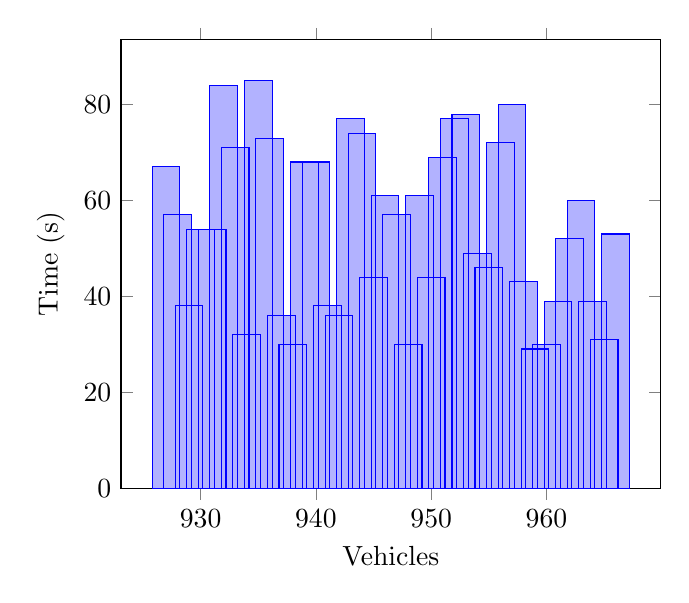
\begin{tikzpicture}
\begin{axis}[
legend style={anchor=west},
xlabel=Vehicles,
ylabel=Time (s),
ymin=0,
ybar,
]
\addplot coordinates {
(951, 69)
(948, 30)
(949, 61)
(946, 61)
(947, 57)
(944, 74)
(945, 44)
(942, 36)
(943, 77)
(940, 68)
(941, 38)
(927, 67)
(938, 30)
(933, 71)
(932, 84)
(931, 54)
(930, 54)
(937, 36)
(935, 85)
(934, 32)
(928, 57)
(929, 38)
(952, 77)
(939, 68)
(964, 39)
(965, 31)
(966, 53)
(960, 30)
(961, 39)
(962, 52)
(963, 60)
(936, 73)
(956, 72)
(953, 78)
(959, 29)
(958, 43)
(950, 44)
(955, 46)
(954, 49)
(957, 80)
};

\end{axis}
\end{tikzpicture}
\label{tik:time:100:13}
\caption{100 percent diving with GSC on route $13$}
\end{figure}
